% 2026年北京高考数学第10题：平面四边形连杆机构与圆
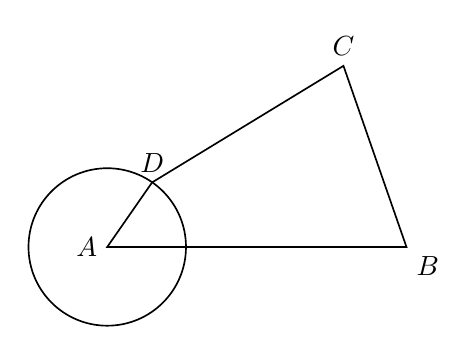
\begin{tikzpicture}[>=stealth,line width=0.6pt,font=\normalsize]
  \coordinate (A) at (0,0);
  \coordinate (B) at (3.8,0);
  \coordinate (D) at (0.57,0.82);
  \coordinate (C) at (3.0,2.3);

  % 圆 A
  \draw (A) circle (1.0cm);

  % 连杆边
  \draw (A) -- (B) -- (C) -- (D) -- cycle;

  % 顶点标注
  \node[left] at (A) {$A$};
  \node[below right] at (B) {$B$};
  \node[above] at (C) {$C$};
  \node[above] at (D) {$D$};
\end{tikzpicture}
